\begin{figure}[H]
    \centering
    
    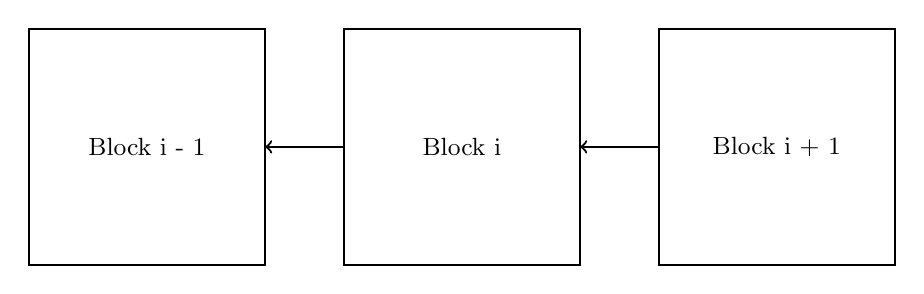
\begin{tikzpicture}[
        node distance=2cm,
        every node/.style={
            font=\small 
        }
    ]
        % Block 1
        \begin{scope}[xshift=0cm]
            \draw[thick] (0, 0) rectangle (3, 3);

            \node at (1.5, 1.5) {Block i - 1};
        \end{scope}

        % Block 2
        \begin{scope}[xshift=4cm]
            \draw[thick] (0, 0) rectangle (3, 3);

            \node at (1.5, 1.5) {Block i};
        \end{scope}

        % Block 3
        \begin{scope}[xshift=8cm]
            \draw[thick] (0, 0) rectangle (3, 3);

            \node at (1.5, 1.5) {Block i + 1};
        \end{scope}

        \draw[<-, thick] (3,1.5) -- (4,1.5);

        \draw[<-, thick] (7,1.5) -- (8,1.5);
        
    \end{tikzpicture}
    
    \caption{Blockchain architecture}
    
    \label{fig:blockchain_architecture}
\end{figure}